% ============================================================
%  Anexo II - Estimación del tamaño y esfuerzo del proyecto
%  Sistema de Gestión Documental mediante Blockchain
%  Compilar con: lualatex AnexoII_EstimacionPlanificacion.tex
% ============================================================

% ============================================================
% NOTA ENCODING (2026-03-27): Archivo corregido a UTF-8.
% Los caracteres acentuados (tildes) habian sido danados por
% una operacion de I/O con codificacion ISO-8859-1 en PS5.
% Patron 1 (AnexoI): U+FFFD para a/e/i/n/u; '?' para 'o'.
%   Solucion: diccionario de contexto + regex (fix_accents_v2.py, fix3.py).
% Patron 2 (AnexoII-V): todos los acentos como '?' literal.
%   Solucion: vacabulario de 462 entradas (fix_annexes_all.py, fix_final.py).
% REGLA: Siempre usar Python 3 + io.open(path,'w',encoding='utf-8').
%        NUNCA usar Set-Content de PowerShell 5 (anade BOM o rompe tildes).
% ============================================================
\documentclass[11pt, a4paper]{article}

\usepackage{fontspec}
\usepackage[spanish]{babel}
\usepackage{graphicx}
\usepackage{float}
\usepackage{amsmath}
\usepackage{amssymb}
\usepackage{xcolor}
\usepackage[protrusion=true,expansion=false]{microtype}
\usepackage{longtable}
\usepackage{array}
\usepackage{booktabs}
\usepackage{multirow}
\usepackage{enumitem}
\usepackage{pgfgantt}
\usepackage[
    colorlinks = true,
    linkcolor  = black,
    urlcolor   = black,
    citecolor  = black
]{hyperref}

\usepackage{geometry}
\geometry{
    left       = 2.5cm,
    right      = 2.5cm,
    top        = 3cm,
    bottom     = 2.5cm,
    headheight = 55pt,
    headsep    = 0.8cm
}

\usepackage{fancyhdr}
\pagestyle{fancy}
\fancyhf{}

\lhead{
\includegraphics[height=1.25cm]{USAL-Logo-3820702873.png}}
\rhead{\shortstack[r]{\fontsize{10}{12}\selectfont\textbf{\tituloInforme}\\[-1pt]\fontsize{10}{12}\selectfont\subtituloInforme}}

\renewcommand{\headrulewidth}{0pt}
\renewcommand{\footrulewidth}{0pt}

\cfoot{%
    \color{gray}\rule[0.5ex]{0.4\textwidth}{0.8pt}%
    \hspace{0.5cm}%
    \textcolor{black}{\textbf{\thepage}}%
    \hspace{0.5cm}%
    \color{gray}\rule[0.5ex]{0.4\textwidth}{0.8pt}%
}

\newcommand{\tituloInforme}{Anexo II: Estimación del tamaño y esfuerzo}
\newcommand{\subtituloInforme}{Sistema de Gestión Documental mediante Blockchain}
\newcommand{\asignatura}{Trabajo de Fin de Grado}
\newcommand{\autorUno}{David Pérez Velasco}
\newcommand{\tutorUno}{Gabriel Villarrubia González}
\newcommand{\tutorDos}{Sergio García González}

\graphicspath{{diagramas/}}
\begin{document}

\begin{titlepage}
    \centering
    \vspace*{1.5cm}

    {\scshape\LARGE Universidad de Salamanca \par}
    \vspace{1cm}
    {\scshape\Large Grado en Ingeniería Informática \par}
    \vspace{1.5cm}

    {\huge\bfseries \tituloInforme \par}
    \vspace{0.5cm}
    {\Large\bfseries \subtituloInforme \par}
    \vspace{1.8cm}

    
\includegraphics[width=0.28\textwidth]{USAL-Logo-3820702873.png}

    \vspace{2.2cm}

    {\Large\itshape \autorUno \par}
    \vspace{1.5cm}
    {\large Tutores: \par}
    \vspace{0.3cm}
    {\large \tutorUno \par}
    \vspace{0.2cm}
    {\large \tutorDos \par}

    \vspace{2cm}
    {\large Julio 2026}
    \vspace{0.5cm}

    \asignatura

    \vspace{1cm}
\end{titlepage}

\setcounter{page}{2}
\pagestyle{fancy}

\tableofcontents
\newpage

\listoffigures
\newpage

\listoftables
\newpage

\section{Introducción}

En este anexo se recoge la estimación del esfuerzo y la planificación temporal de \textbf{DocumentChain}, el sistema de gestión documental con blockchain que constituye este TFG. Para la estimación se ha utilizado la herramienta \textbf{EZEstimate}, que se apoya en los \textbf{Puntos de Caso de Uso (UCP -- \textit{Use Case Points})}, y como marco de trabajo se ha seguido el \textbf{Proceso Unificado (PU)}.

El método UCP arranca a partir de los actores y casos de uso identificados y los ajusta con factores de complejidad técnica y del entorno. Es un enfoque sencillo pero útil para hacerse una idea realista del esfuerzo en proyectos con componentes heterogéneos. El Proceso Unificado, por su parte, divide el trabajo en cuatro fases (\textit{Inicio}, \textit{Elaboración}, \textit{Construcción} y \textit{Transición}), cada una con sus propias iteraciones. Esto ayuda a ir abordando la complejidad poco a poco.

El proyecto tiene una complejidad particular porque mezcla cuatro tecnologías muy distintas entre sí: un \textit{backend} REST en Node.js, una base de datos PostgreSQL, almacenamiento descentralizado sobre IPFS mediante un nodo Kubo autoalojado y un \textit{smart contract} en Solidity sobre Ethereum. Tener que coordinar cuatro subsistemas tan dispares justifica tanto la elección del Proceso Unificado como el esfuerzo de estimación que se detalla a continuación.

La estimación se hace sobre el \textbf{catálogo de 39 casos de uso principales}, en coherencia con el Anexo I. Los 4 casos restantes del catálogo funcional completo (43 UC) se integran como subflujos de estos 39, por lo que no añaden peso UCP independiente al no requerir transacciones ni flujos de análisis diferenciados. Así se evita contar dos veces el mismo esfuerzo en el cálculo UCP.

El mapeo detallado entre qué operación se integró en qué UC principal está en el Anexo I. De esta forma, la estimación, las especificaciones y los diagramas de paquetes comparten el mismo criterio, por lo que se garantiza la coherencia entre los distintos anexos del proyecto.

\section{Estudio de viabilidad del proyecto}

\subsection{Objetivos del sistema}

El desarrollo de DocumentChain sigue las cuatro fases fundamentales del Proceso Unificado, organizadas con dos iteraciones cada una, lo que permite abordar progresivamente la complejidad del sistema:

\begin{description}[leftmargin=2cm, style=nextline]
    \item[\textbf{Inicio}] Su objetivo es establecer el alcance del proyecto, identificar a los actores y sus interacciones principales, y evaluar la viabilidad del sistema. En la primera iteración se realiza un contacto inicial con el problema y el dominio; en la segunda se definen con precisión los objetivos, actores y casos de uso más relevantes, y se elabora la planificación inicial.

    \item[\textbf{Elaboración}] Su objetivo es estabilizar la arquitectura del sistema, completar el análisis de requisitos y reducir los riesgos técnicos. En la primera iteración se especifican en detalle los requisitos (IRQ, NFR) y se diseña la arquitectura general; en la segunda se diseñan los componentes más complejos (smart contract, cifrado híbrido de documentos y protección de claves) y se elaboran los diagramas UML y la documentación técnica.

    \item[\textbf{Construcción}] Su objetivo es implementar el sistema completo de forma iterativa. La primera iteración abarca los subsistemas centrales: autenticación, documentos, versionado, firmas, compartición y el frontend básico. La segunda iteración añade funcionalidades avanzadas: estadísticas, auditoría, administración, notificaciones y ajustes de rendimiento y seguridad.

    \item[\textbf{Transición}] Su objetivo es desplegar el sistema en el entorno de producción, validarlo con usuarios reales y cerrar el proyecto. La primera iteración contempla el despliegue completo y las pruebas finales; la segunda el cierre de la documentación académica y la entrega del TFG.
\end{description}

\subsection{Factores de complejidad técnica y del entorno}

\subsubsection{Factores de complejidad técnica}

El método UCP define 13 factores técnicos (T1--T13) que impactan la complejidad del proyecto, detallados en la Tabla~\ref{tab:factores-tecnicos}. Cada factor se puntúa de 0 (sin impacto) a 5 (máximo impacto) y se multiplica por su peso predefinido para obtener el subtotal.

\begin{longtable}{|p{0.8cm}|p{7.5cm}|p{1.3cm}|p{1.8cm}|p{2cm}|}
\hline
\textbf{ID} & \textbf{Factor} & \textbf{Peso} & \textbf{Valoración} & \textbf{Subtotal} \\
\hline
\endfirsthead
\hline
\textbf{ID} & \textbf{Factor} & \textbf{Peso} & \textbf{Valoración} & \textbf{Subtotal} \\
\hline
\endhead
T1 & Sistema distribuido (Blockchain + IPFS + REST API) & 2.0 & 5 & 10.0 \\
\hline
T2 & Objetivos de rendimiento y tiempos de respuesta & 1.0 & 4 & 4.0 \\
\hline
T3 & Eficiencia del usuario final (UX intuitiva) & 1.0 & 4 & 4.0 \\
\hline
T4 & Procesamiento interno complejo (cifrado híbrido, blockchain) & 1.0 & 5 & 5.0 \\
\hline
T5 & Código reutilizable y modular & 1.0 & 4 & 4.0 \\
\hline
T6 & Facilidad de instalación (Docker Compose) & 0.5 & 3 & 1.5 \\
\hline
T7 & Facilidad de uso (interfaz web intuitiva) & 0.5 & 4 & 2.0 \\
\hline
T8 & Portabilidad (multi-plataforma vía navegador web) & 2.0 & 4 & 8.0 \\
\hline
T9 & Facilidad de cambio y mantenimiento & 1.0 & 4 & 4.0 \\
\hline
T10 & Concurrencia (múltiples usuarios simultáneos) & 1.0 & 4 & 4.0 \\
\hline
T11 & Seguridad especial (cifrado de documentos, control de acceso e inmutabilidad blockchain) & 1.0 & 5 & 5.0 \\
\hline
T12 & Acceso de terceros (wallets compatibles, nodos IPFS, Ethereum) & 1.0 & 5 & 5.0 \\
\hline
T13 & Facilidades de formación para usuarios & 1.0 & 3 & 3.0 \\
\hline
\multicolumn{4}{|r|}{\textbf{Total Factor Técnico (TF):}} & \textbf{59.5} \\
\hline
\caption{Factores de complejidad técnica (T1--T13)}\label{tab:factores-tecnicos}
\end{longtable}

\vspace{0.5em}
\noindent El \textbf{Factor de Complejidad Técnica (TCF)} se calcula como:

\begin{equation}
\text{TCF} = 0{,}6 + (0{,}01 \times \text{TF}) = 0{,}6 + (0{,}01 \times 59{,}5) = \mathbf{1{,}195}
\end{equation}

Un TCF superior a 1,0 indica complejidad técnica elevada, consecuencia directa de la integración de blockchain, criptografía avanzada y almacenamiento distribuido.

\subsubsection{Factores del entorno}

El método UCP define 8 factores del entorno (E1--E8) relacionados con el equipo y el contexto de desarrollo, recogidos en la Tabla~\ref{tab:factores-entorno}. Los factores E7 y E8 tienen peso negativo, penalizando escenarios desfavorables.

\begin{longtable}{|p{0.8cm}|p{7.5cm}|p{1.3cm}|p{1.8cm}|p{2cm}|}
\hline
\textbf{ID} & \textbf{Factor} & \textbf{Peso} & \textbf{Valoración} & \textbf{Subtotal} \\
\hline
\endfirsthead
\hline
\textbf{ID} & \textbf{Factor} & \textbf{Peso} & \textbf{Valoración} & \textbf{Subtotal} \\
\hline
\endhead
E1 & Familiaridad con el modelo de proyecto (TFG académico) & 1.5 & 3 & 4.5 \\
\hline
E2 & Experiencia en la aplicación (blockchain, nuevo dominio) & 0.5 & 2 & 1.0 \\
\hline
E3 & Experiencia en orientación a objetos (TypeScript) & 1.0 & 4 & 4.0 \\
\hline
E4 & Capacidad del analista líder (autónomo, tutorizado) & 0.5 & 3 & 1.5 \\
\hline
E5 & Motivación del equipo (alta --- proyecto TFG personal) & 1.0 & 5 & 5.0 \\
\hline
E6 & Estabilidad de requisitos (bien definidos, pocos cambios) & 2.0 & 4 & 8.0 \\
\hline
E7 & Personal a tiempo parcial (estudiante, 6h/día) & -1.0 & 3 & -3.0 \\
\hline
E8 & Dificultad del lenguaje (TypeScript + Solidity) & -1.0 & 3 & -3.0 \\
\hline
\multicolumn{4}{|r|}{\textbf{Total Factor Ambiental (EF):}} & \textbf{18.0} \\
\hline
\caption{Factores del entorno (E1--E8)}\label{tab:factores-entorno}
\end{longtable}

\vspace{0.5em}
\noindent El \textbf{Factor de Complejidad del Entorno (ECF)} se calcula como:

\begin{equation}
\text{ECF} = 1{,}4 + (-0{,}03 \times \text{EF}) = 1{,}4 + (-0{,}03 \times 18{,}0) = \mathbf{0{,}86}
\end{equation}

Un ECF inferior a 1,0 refleja factores negativos como la curva de aprendizaje en blockchain y la dedicación a tiempo parcial, que reducen ligeramente la productividad estimada.

\subsection{Lista de casos de uso y representación de actores}

El sistema DocumentChain cuenta con \textbf{5 actores} y un \textbf{catálogo de 39 casos de uso principales}. Para el cálculo UCP de este anexo se ponderan esos mismos 39 UC, mientras que las operaciones complementarias quedan absorbidas como variantes de los flujos principales. Para facilitar la lectura, los diagramas de casos de uso se presentan agrupados por áreas funcionales. La Figura~\ref{fig:uc_acceso} muestra el paquete de Gestión de Acceso.

\begin{figure}[H]
    \centering
    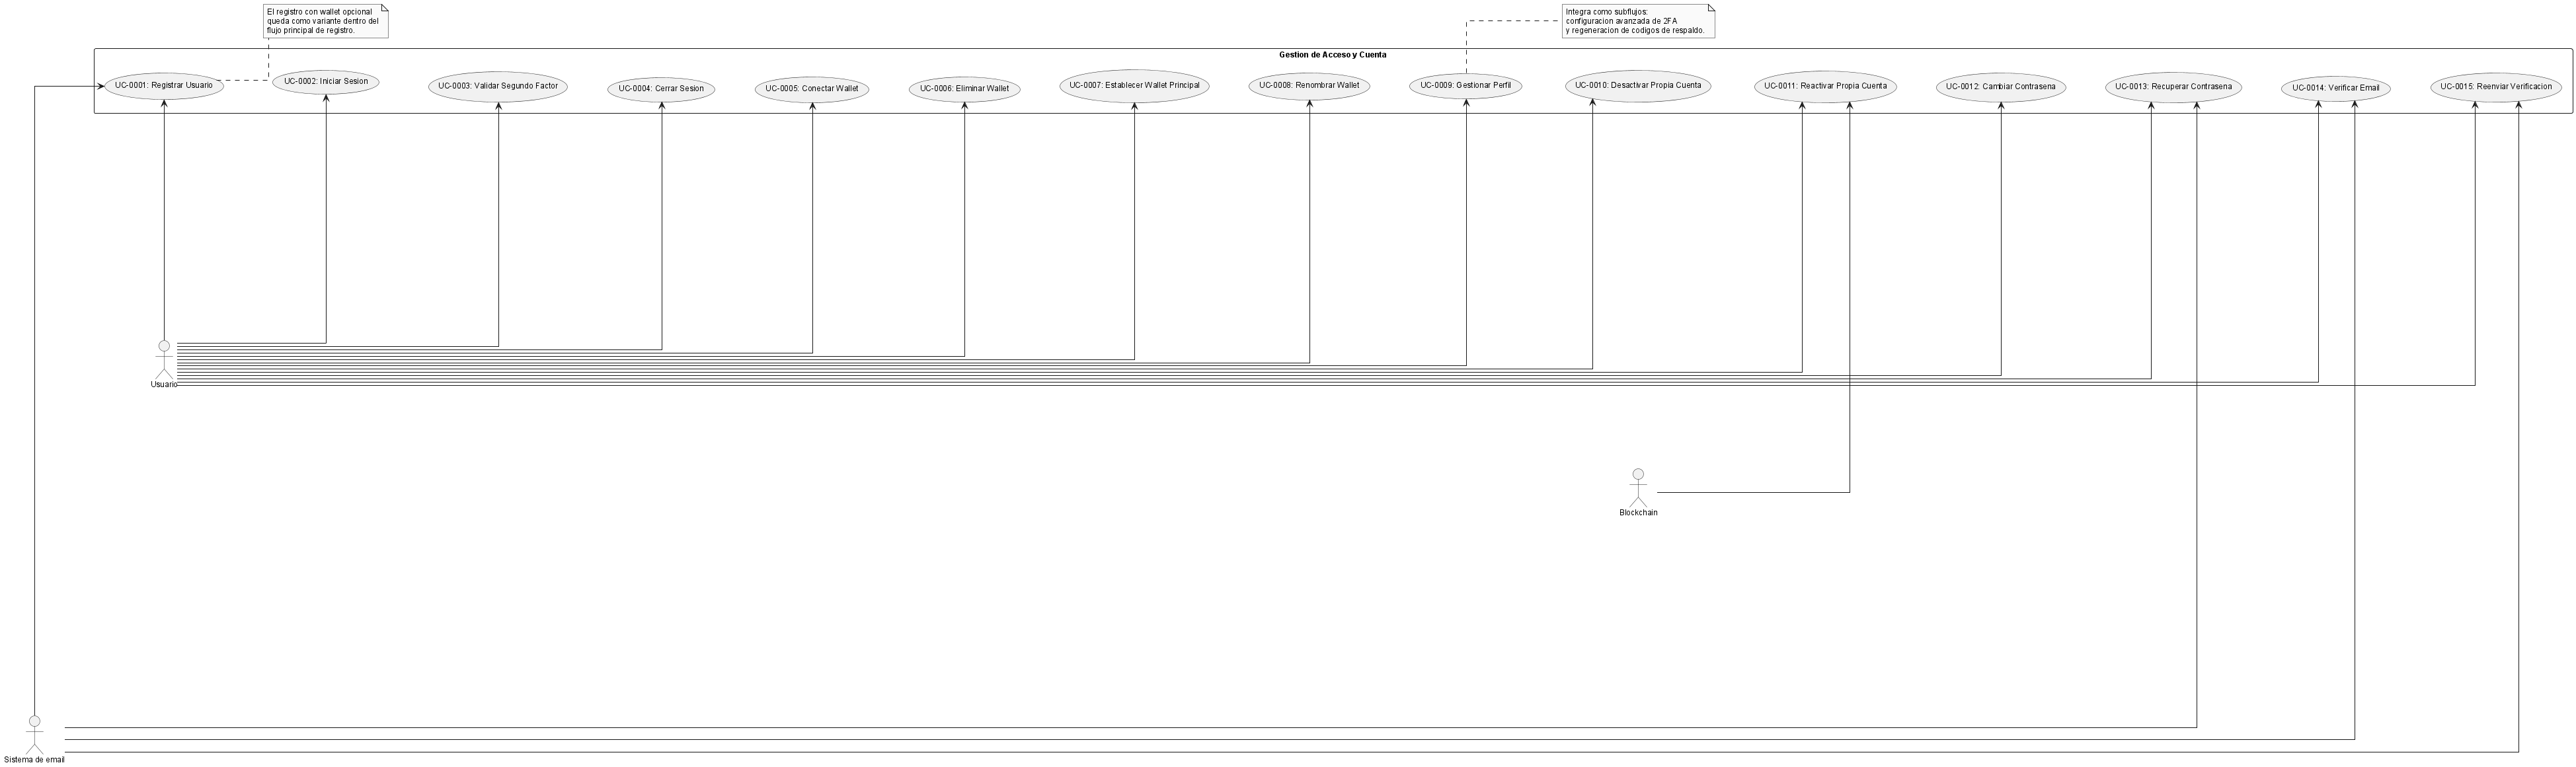
\includegraphics[width=0.98\linewidth]{diagramas/uc_acceso.png}
    \caption{Diagrama de casos de uso: Paquete de Gestión de Acceso}
    \label{fig:uc_acceso}
\end{figure}

La Figura~\ref{fig:uc_documentos} presenta el paquete de Gestión de Documentos.
\begin{figure}[H]
    \centering
    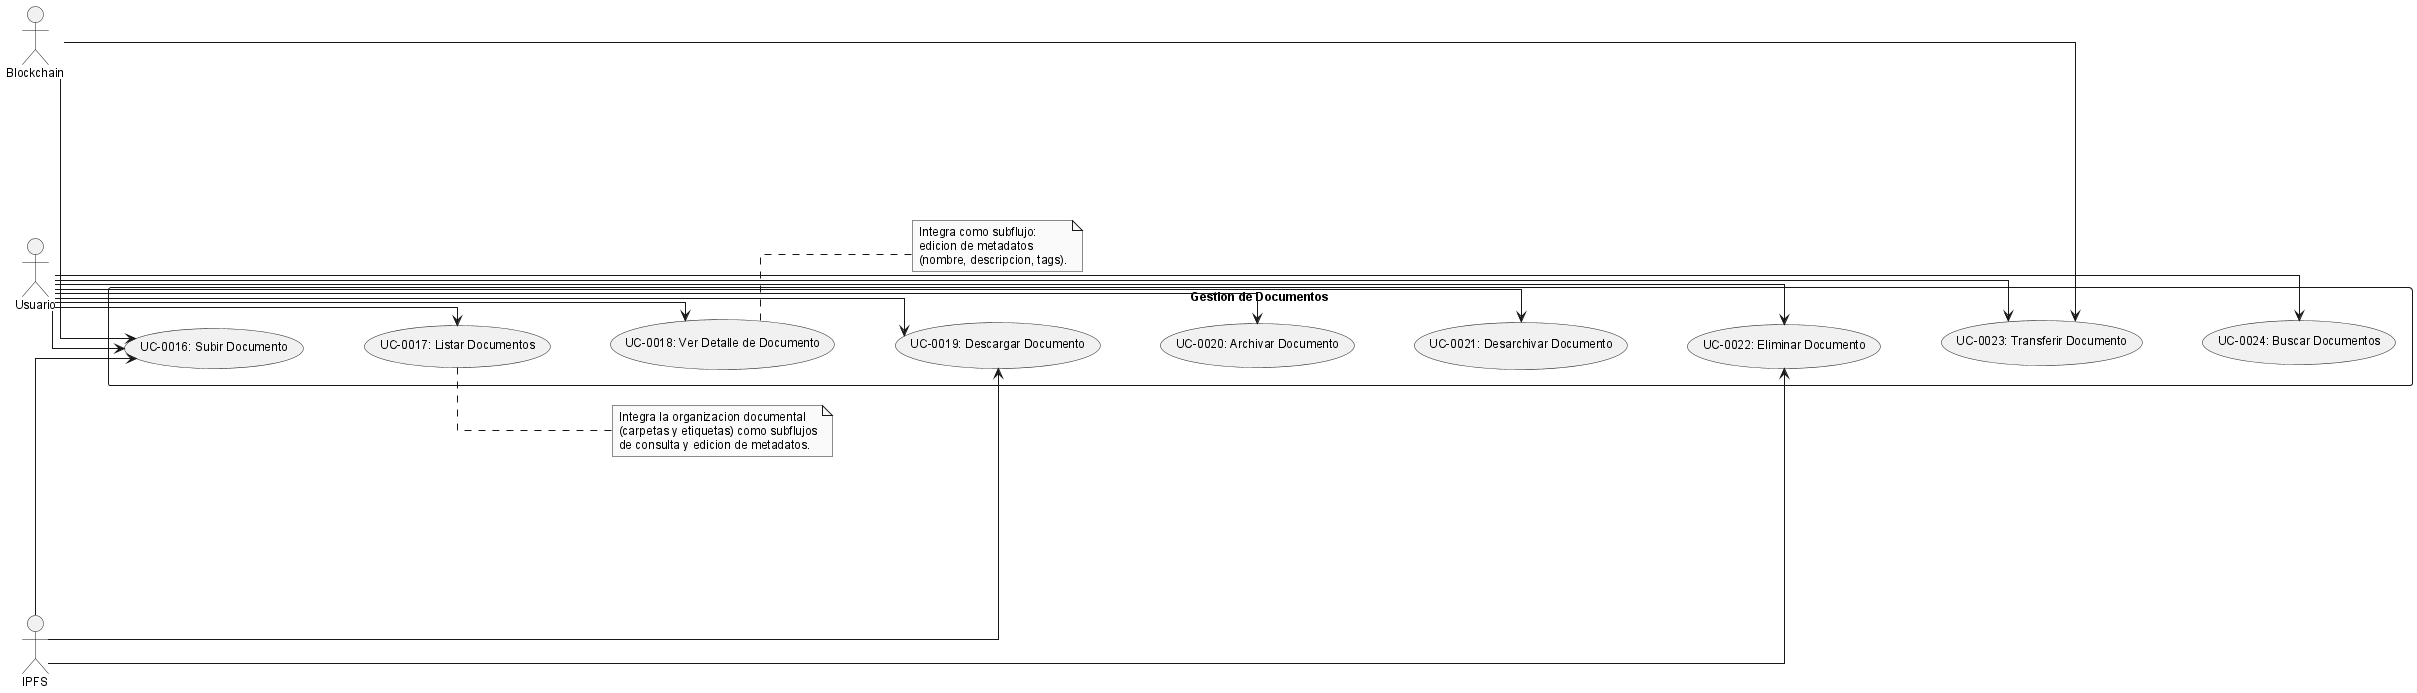
\includegraphics[width=0.98\linewidth]{diagramas/uc_documentos.png}
    \caption{Diagrama de casos de uso: Paquete de Gestión de Documentos}
    \label{fig:uc_documentos}
\end{figure}

La Figura~\ref{fig:uc_versiones} ilustra el paquete de Gestión de Versiones.
\begin{figure}[H]
    \centering
    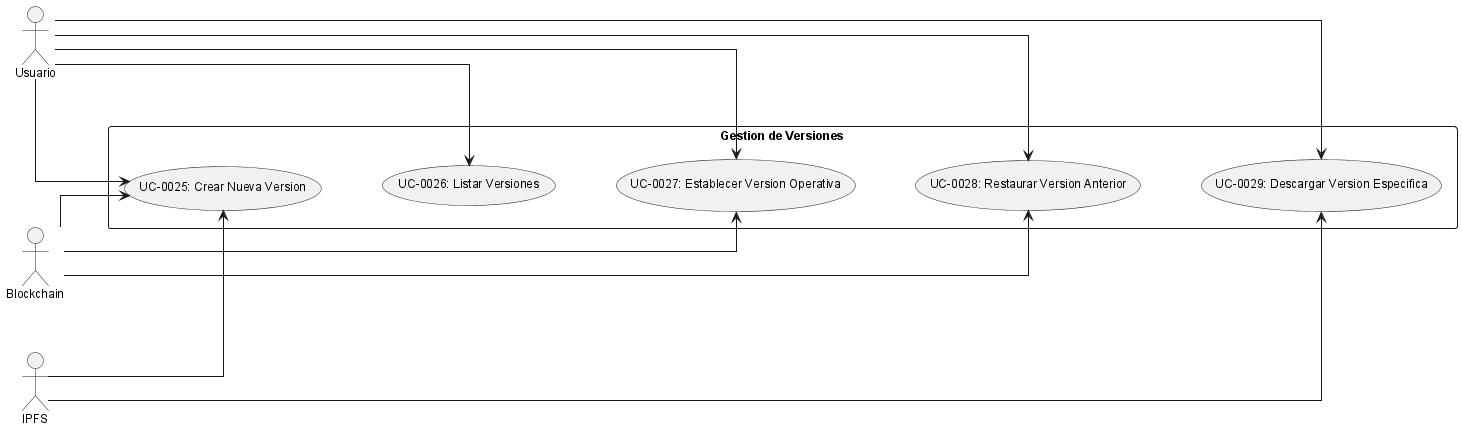
\includegraphics[width=0.95\linewidth]{diagramas/uc_versiones.png}
    \caption{Diagrama de casos de uso: Paquete de Gestión de Versiones}
    \label{fig:uc_versiones}
\end{figure}

En la Figura~\ref{fig:uc_firmas} se detalla el paquete de Gestión de Firmas.
\begin{figure}[H]
    \centering
    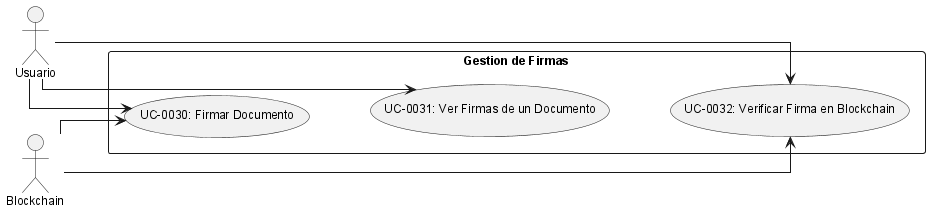
\includegraphics[width=0.92\linewidth]{diagramas/uc_firmas.png}
    \caption{Diagrama de casos de uso: Paquete de Gestión de Firmas}
    \label{fig:uc_firmas}
\end{figure}

La Figura~\ref{fig:uc_comparticion} corresponde al paquete de Gestión de Compartición.
\begin{figure}[H]
    \centering
    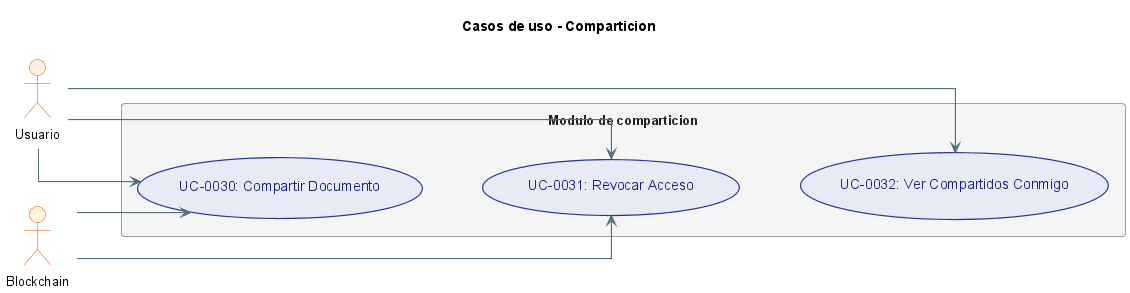
\includegraphics[width=0.95\linewidth]{diagramas/uc_comparticion.png}
    \caption{Diagrama de casos de uso: Paquete de Gestión de Compartición}
    \label{fig:uc_comparticion}
\end{figure}

La Figura~\ref{fig:uc_auditoria} recoge el paquete de Auditoría y Estadísticas.
\begin{figure}[H]
    \centering
    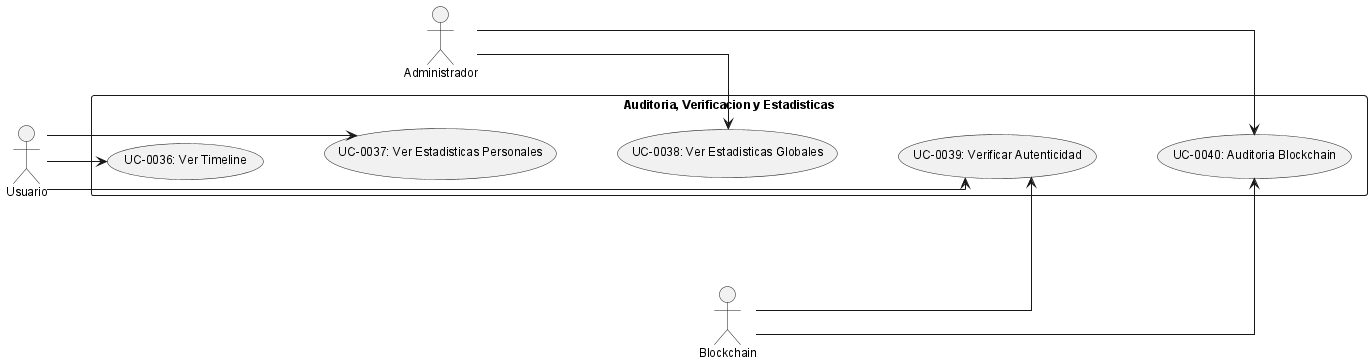
\includegraphics[width=0.98\linewidth]{diagramas/uc_auditoria.png}
    \caption{Diagrama de casos de uso: Paquete de Auditoría y Estadísticas}
    \label{fig:uc_auditoria}
\end{figure}

Finalmente, la Figura~\ref{fig:uc_administracion} muestra el paquete de Administración.
\begin{figure}[H]
    \centering
    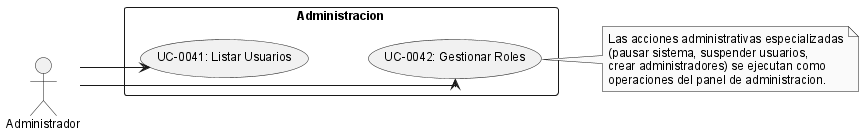
\includegraphics[width=0.88\linewidth]{diagramas/uc_administracion.png}
    \caption{Diagrama de casos de uso: Paquete de Administración}
    \label{fig:uc_administracion}
\end{figure}

\subsection{Actores del sistema}

Los actores del sistema se clasifican según su complejidad de interacción, como se resume en la Tabla~\ref{tab:actores}:

\begin{itemize}
    \item \textbf{Simple} (peso 1): Sistema externo con API definida
    \item \textbf{Medio} (peso 2): Sistema con protocolo o interfaz textual
    \item \textbf{Complejo} (peso 3): Usuario a través de interfaz gráfica
\end{itemize}

\begin{table}[H]
\centering
\begin{tabular}{|l|p{7cm}|l|c|}
\hline
\textbf{ID} & \textbf{Actor} & \textbf{Tipo} & \textbf{Peso} \\
\hline
ACT-01 & Usuario registrado (interfaz web compleja) & Complejo & 3 \\
\hline
ACT-02 & Administrador (interfaz web de administración) & Complejo & 3 \\
\hline
ACT-03 & Smart Contract DocumentRegistry (API JSON-RPC) & Simple & 1 \\
\hline
ACT-04 & Nodo IPFS autoalojado (API HTTP) & Simple & 1 \\
\hline
ACT-05 & Sistema de Email SMTP & Medio & 2 \\
\hline
\multicolumn{3}{|r|}{\textbf{Total Peso de Actores (UAW):}} & \textbf{10} \\
\hline
\end{tabular}
    \caption{Clasificación de actores del sistema}\label{tab:actores}
\end{table}

La herramienta EZEstimate refleja esta clasificación de actores, como se observa en la Figura~\ref{fig:ezestimate-actors}.
\begin{figure}[H]
    \centering
    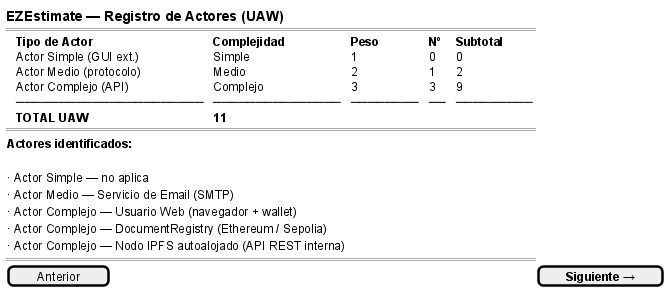
\includegraphics[width=0.88\linewidth]{diagramas/ezestimate-actors.png}
    \caption{EZEstimate --- Pantalla de registro y ponderación de actores (UAW)}
    \label{fig:ezestimate-actors}
\end{figure}

\subsection{Casos de uso}

Los casos de uso se clasifican según el número de transacciones (interacciones) necesarias para completarlos:

\begin{itemize}
    \item \textbf{Simple} (1--3 transacciones, peso 5)
    \item \textbf{Medio} (4--7 transacciones, peso 10)
    \item \textbf{Complejo} (8 o más transacciones, peso 15)
\end{itemize}

\subsubsection*{Paquete: Gestión de Acceso y Cuenta}

\begin{longtable}{|p{1.8cm}|p{6.5cm}|p{3cm}|p{1.5cm}|}
\hline
\textbf{ID} & \textbf{Caso de Uso} & \textbf{Complejidad (Tx)} & \textbf{Peso} \\
\hline
\endfirsthead
\hline
\textbf{ID} & \textbf{Caso de Uso} & \textbf{Complejidad (Tx)} & \textbf{Peso} \\
\hline
\endhead
UC-0001 & Registrar Usuario & Complejo (10) & 15 \\
\hline
UC-0002 & Iniciar Sesión & Medio (6) & 10 \\
\hline
UC-0003 & Cerrar Sesión & Simple (2) & 5 \\
\hline
UC-0004 & Conectar Wallet & Medio (5) & 10 \\
\hline
UC-0005 & Eliminar Wallet & Simple (2) & 5 \\
\hline
UC-0006 & Establecer Wallet Principal & Medio (4) & 10 \\
\hline
UC-0007 & Renombrar Wallet & Simple (3) & 5 \\
\hline
UC-0008 & Gestionar Perfil y Notificaciones & Medio (5) & 10 \\
\hline
UC-0009 & Eliminar Cuenta & Medio (5) & 10 \\
\hline
UC-0010 & Cambiar Contraseña & Medio (5) & 10 \\
\hline
UC-0011 & Verificar Email & Simple (2) & 5 \\
\hline
UC-0012 & Reenviar Verificación de Email & Simple (2) & 5 \\
\hline
\multicolumn{3}{|r|}{\textbf{Subtotal Gestión de Acceso y Cuenta:}} & \textbf{100} \\
\hline
\caption{Casos de uso --- Gestión de Acceso y Cuenta}\label{tab:uc-acceso}
\end{longtable}

\subsubsection*{Paquete: Gestión de Documentos}

\begin{longtable}{|p{1.8cm}|p{6.5cm}|p{3cm}|p{1.5cm}|}
\hline
\textbf{ID} & \textbf{Caso de Uso} & \textbf{Complejidad (Tx)} & \textbf{Peso} \\
\hline
\endfirsthead
\hline
\textbf{ID} & \textbf{Caso de Uso} & \textbf{Complejidad (Tx)} & \textbf{Peso} \\
\hline
\endhead
UC-0013 & Subir Documento & Complejo (12) & 15 \\
\hline
UC-0014 & Listar Documentos & Medio (5) & 10 \\
\hline
UC-0015 & Ver Detalle de Documento & Medio (4) & 10 \\
\hline
UC-0016 & Descargar Documento & Complejo (9) & 15 \\
\hline
UC-0017 & Archivar Documento & Medio (5) & 10 \\
\hline
UC-0018 & Desarchivar Documento & Medio (4) & 10 \\
\hline
UC-0019 & Eliminar Documento & Medio (5) & 10 \\
\hline
UC-0020 & Transferir Documento & Medio (7) & 10 \\
\hline
UC-0021 & Buscar Documentos & Complejo (8) & 15 \\
\hline
\multicolumn{3}{|r|}{\textbf{Subtotal Gestión de Documentos:}} & \textbf{105} \\
\hline
\caption{Casos de uso --- Gestión de Documentos}\label{tab:uc-documentos}
\end{longtable}

\subsubsection*{Paquete: Gestión de Versiones}

\begin{longtable}{|p{1.8cm}|p{6.5cm}|p{3cm}|p{1.5cm}|}
\hline
\textbf{ID} & \textbf{Caso de Uso} & \textbf{Complejidad (Tx)} & \textbf{Peso} \\
\hline
\endfirsthead
\hline
\textbf{ID} & \textbf{Caso de Uso} & \textbf{Complejidad (Tx)} & \textbf{Peso} \\
\hline
\endhead
UC-0022 & Crear Nueva Versión & Complejo (10) & 15 \\
\hline
UC-0023 & Listar Versiones & Simple (2) & 5 \\
\hline
UC-0024 & Establecer Versión Operativa & Simple (2) & 5 \\
\hline
UC-0025 & Restaurar Versión Anterior & Medio (7) & 10 \\
\hline
UC-0026 & Descargar Versión Específica & Medio (5) & 10 \\
\hline
\multicolumn{3}{|r|}{\textbf{Subtotal Gestión de Versiones:}} & \textbf{45} \\
\hline
\caption{Casos de uso --- Gestión de Versiones}\label{tab:uc-versiones}
\end{longtable}

\subsubsection*{Paquete: Gestión de Firmas}

\begin{longtable}{|p{1.8cm}|p{6.5cm}|p{3cm}|p{1.5cm}|}
\hline
\textbf{ID} & \textbf{Caso de Uso} & \textbf{Complejidad (Tx)} & \textbf{Peso} \\
\hline
\endfirsthead
\hline
\textbf{ID} & \textbf{Caso de Uso} & \textbf{Complejidad (Tx)} & \textbf{Peso} \\
\hline
\endhead
UC-0027 & Firmar Documento & Complejo (11) & 15 \\
\hline
UC-0028 & Ver Firmas de un Documento & Simple (2) & 5 \\
\hline
UC-0029 & Verificar Firma del Usuario & Medio (6) & 10 \\
\hline
\multicolumn{3}{|r|}{\textbf{Subtotal Gestión de Firmas:}} & \textbf{30} \\
\hline
\caption{Casos de uso --- Gestión de Firmas}\label{tab:uc-firmas}
\end{longtable}

\subsubsection*{Paquete: Gestión de Compartición}

\begin{longtable}{|p{1.8cm}|p{6.5cm}|p{3cm}|p{1.5cm}|}
\hline
\textbf{ID} & \textbf{Caso de Uso} & \textbf{Complejidad (Tx)} & \textbf{Peso} \\
\hline
\endfirsthead
\hline
\textbf{ID} & \textbf{Caso de Uso} & \textbf{Complejidad (Tx)} & \textbf{Peso} \\
\hline
\endhead
UC-0030 & Compartir Documento & Complejo (10) & 15 \\
\hline
UC-0031 & Revocar Acceso a Documento & Medio (5) & 10 \\
\hline
UC-0032 & Ver Documentos Compartidos Conmigo & Medio (4) & 10 \\
\hline
\multicolumn{3}{|r|}{\textbf{Subtotal Gestión de Compartición:}} & \textbf{35} \\
\hline
\caption{Casos de uso --- Gestión de Compartición}\label{tab:uc-comparticion}
\end{longtable}

\subsubsection*{Paquete: Auditoría, Verificación y Estadísticas}

\begin{longtable}{|p{1.8cm}|p{6.5cm}|p{3cm}|p{1.5cm}|}
\hline
\textbf{ID} & \textbf{Caso de Uso} & \textbf{Complejidad (Tx)} & \textbf{Peso} \\
\hline
\endfirsthead
\hline
\textbf{ID} & \textbf{Caso de Uso} & \textbf{Complejidad (Tx)} & \textbf{Peso} \\
\hline
\endhead
UC-0033 & Ver Timeline de Documento & Medio (5) & 10 \\
\hline
UC-0034 & Ver Estadísticas Personales & Medio (5) & 10 \\
\hline
UC-0035 & Ver Estadísticas Globales del Sistema & Medio (5) & 10 \\
\hline
UC-0036 & Verificar Autenticidad de Documento & Medio (6) & 10 \\
\hline
UC-0037 & Auditoría Blockchain & Medio (6) & 10 \\
\hline
\multicolumn{3}{|r|}{\textbf{Subtotal Auditoría, Verificación y Estadísticas:}} & \textbf{50} \\
\hline
\caption{Casos de uso --- Auditoría, Verificación y Estadísticas}\label{tab:uc-auditoria}
\end{longtable}

\subsubsection*{Paquete: Administración}

\begin{longtable}{|p{1.8cm}|p{6.5cm}|p{3cm}|p{1.5cm}|}
\hline
\textbf{ID} & \textbf{Caso de Uso} & \textbf{Complejidad (Tx)} & \textbf{Peso} \\
\hline
\endfirsthead
\hline
\textbf{ID} & \textbf{Caso de Uso} & \textbf{Complejidad (Tx)} & \textbf{Peso} \\
\hline
\endhead
UC-0038 & Listar Usuarios & Complejo (10) & 15 \\
\hline
UC-0039 & Gestionar Roles de Usuario & Medio (5) & 10 \\
\hline
\multicolumn{3}{|r|}{\textbf{Subtotal Administración:}} & \textbf{25} \\
\hline
\caption{Casos de uso --- Administración}\label{tab:uc-administracion}
\end{longtable}

\subsubsection*{Resumen de clasificación}

El resumen de la clasificación de los 39 casos de uso se presenta en la Tabla~\ref{tab:uucw-resumen}.
\begin{table}[H]
\centering
\begin{tabular}{|l|c|c|c|}
\hline
\textbf{Complejidad} & \textbf{Cantidad} & \textbf{Peso unitario} & \textbf{Total} \\
\hline
Simple (1--3 Tx) & 8 & 5 & 40 \\
\hline
Medio (4--7 Tx) & 23 & 10 & 230 \\
\hline
Complejo (8+ Tx) & 8 & 15 & 120 \\
\hline
\textbf{Total ponderado (UUCW)} & \textbf{39} & --- & \textbf{390} \\
\hline
\end{tabular}
    \caption{Resumen de Pesos de Casos de Uso (UUCW)}\label{tab:uucw-resumen}
\end{table}

La Figura~\ref{fig:ezestimate-uc} muestra la pantalla de EZEstimate con la clasificación de los 39 casos de uso por complejidad.
\begin{figure}[H]
    \centering
    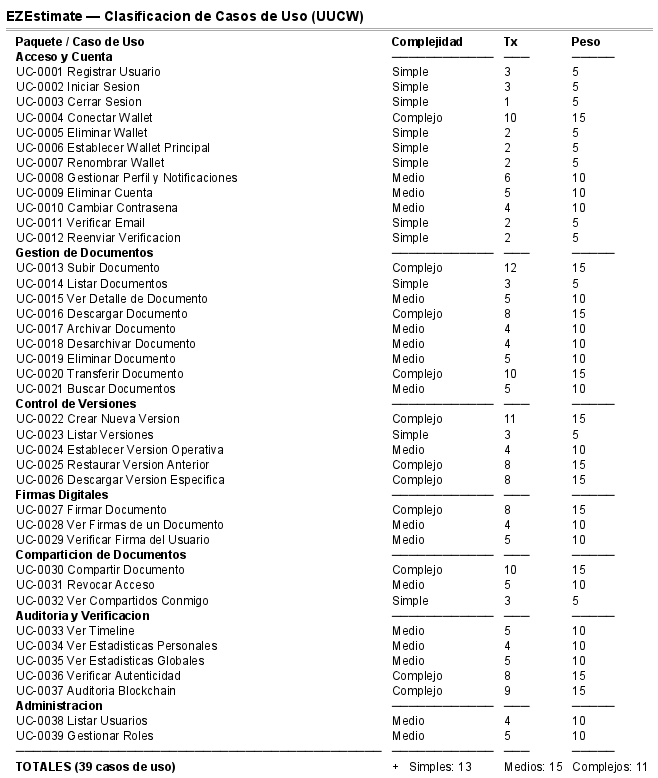
\includegraphics[width=0.92\linewidth]{diagramas/ezestimate-uc-1.png}
    \caption{EZEstimate --- Pantalla de clasificación de casos de uso por complejidad (UUCW)}
    \label{fig:ezestimate-uc}
\end{figure}

\subsection{Conclusión y análisis de resultados}

A partir de los factores y clasificaciones anteriores, se aplica la metodología UCP para obtener los Puntos de Caso de Uso Ajustados (\textit{UCP}):

\begin{align}
\text{UUCP} &= \text{UAW} + \text{UUCW} = 10 + 390 = \mathbf{400} \\[4pt]
\text{UCP} &= \text{UUCP} \times \text{TCF} \times \text{ECF} = 400 \times 1{,}195 \times 0{,}86 \approx \mathbf{411}
\end{align}

Estos valores han sido introducidos en la herramienta \textbf{EZEstimate}, que proporciona una estimación del esfuerzo total considerando los factores de complejidad técnica y del entorno. El resultado obtenido se muestra en la Figura~\ref{fig:ezestimate}.

\begin{figure}[H]
    \centering
    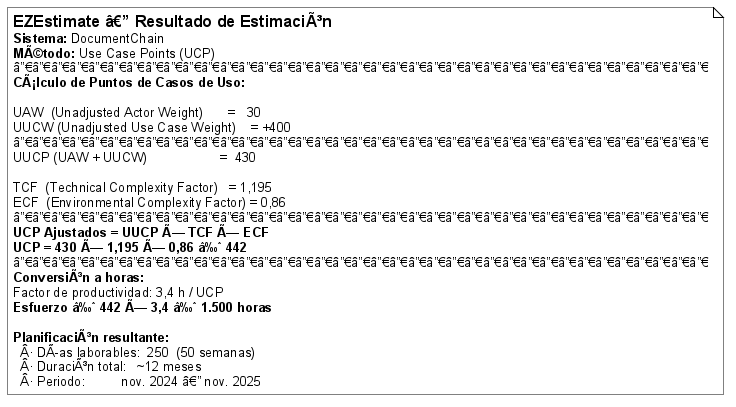
\includegraphics[width=0.92\linewidth]{diagramas/ezestimate.png}
    \caption{EZEstimate --- Factores TCF y ECF con resultado final de la estimación UCP}
    \label{fig:ezestimate}
\end{figure}

El resumen numérico de la estimación se recoge en la Tabla~\ref{tab:estimacion-final}.
\begin{table}[H]
\centering
\begin{tabular}{|l|r|}
\hline
\textbf{Parámetro} & \textbf{Valor} \\
\hline
Puntos de Caso de Uso Sin Ajustar (UUCP) & 400 \\
\hline
Factor de Complejidad Técnica (TCF) & 1{,}195 \\
\hline
Factor del Entorno (ECF) & 0{,}86 \\
\hline
Puntos de Caso de Uso Ajustados (UCP) & 411 \\
\hline
Estimación de esfuerzo total & 1.400 horas \\
\hline
Horas totales estimadas & 1.400 horas \\
\hline
Dedicación real & $\sim$10 h/día (incluye fines de semana) \\
\hline
Duración efectiva & 6 meses \\
\hline
Período de ejecución & 1 dic.\ 2025 -- 15 jun.\ 2026 \\
\hline
\end{tabular}
\caption{Resumen de la estimación de esfuerzo mediante EZEstimate}\label{tab:estimacion-final}
\end{table}

Las 1.400 horas se han calculado aplicando un factor de productividad de \textbf{3,4 h/UCP} ($411 \times 3{,}4 \approx 1.400$), valor que EZEstimate recoge como referencia para proyectos académicos con un único desarrollador. En la práctica, el esfuerzo se ha traducido en \textbf{unos seis meses de trabajo intensivo} (de diciembre de 2025 a mediados de junio de 2026) con una dedicación de unas \textbf{10 horas diarias} de media, fines de semana incluidos.

\section{Planificación temporal}

\subsection{Descripción de tareas, subtareas e hitos}

A continuación se presenta, en la Tabla~\ref{tab:tareas-hitos}, la relación completa de tareas, subtareas e hitos del proyecto DocumentChain, organizada según las fases del Proceso Unificado. Los hitos aparecen en negrita y están identificados por el símbolo $\blacklozenge$.

\begin{longtable}{|p{1cm}|p{5.5cm}|p{1.5cm}|p{5.5cm}|}
\hline
\textbf{Núm.} & \textbf{Tarea o hito} & \textbf{Prec.} & \textbf{Descripción} \\
\hline
\endfirsthead
\hline
\textbf{Núm.} & \textbf{Tarea o hito} & \textbf{Prec.} & \textbf{Descripción} \\
\hline
\endhead
\multicolumn{4}{|c|}{\textit{\textbf{--- FASE: INICIO --- Iteración 1 ---}}} \\
\hline
1 & Reunión inicial con tutores & --- & Primera toma de contacto con el proyecto. Definición del tema, alcance general y tutores asignados. \\
\hline
2 & Análisis del dominio del problema & 1 & Estudio del campo de la gestión documental y del estado del arte blockchain aplicado a documentos. \\
\hline
3 & Estudio de soluciones existentes & 2 & Revisión de sistemas similares (Google Drive, Docusign) y sus carencias respecto a privacidad y trazabilidad. \\
\hline
4 & \textbf{$\blacklozenge$ Fin Iteración 1 (Inicio)} & 3 & Hito que marca el final de la primera iteración de la fase de Inicio. \\
\hline
\multicolumn{4}{|c|}{\textit{\textbf{--- FASE: INICIO --- Iteración 2 ---}}} \\
\hline
5 & Definición del alcance y objetivos & 4 & Especificación de los objetivos del sistema (OBJ-0001 a OBJ-0006) y sus restricciones. \\
\hline
6 & Identificación de actores y UC iniciales & 5 & Identificación preliminar de los 5 actores y los casos de uso más representativos del sistema. \\
\hline
7 & Selección del stack tecnológico & 5 & Evaluación y selección de las tecnologías principales: React, Node.js, PostgreSQL, Solidity, IPFS. \\
\hline
8 & Elaboración de la planificación inicial & 6 & Estimación preliminar del esfuerzo y definición del calendario de trabajo por fases. \\
\hline
9 & \textbf{$\blacklozenge$ Fin Iteración 2 (Inicio)} & 8 & Hito que marca el final de la segunda iteración de la fase de Inicio. \\
\hline
\multicolumn{4}{|c|}{\textit{\textbf{--- FASE: ELABORACIÓN --- Iteración 1 ---}}} \\
\hline
10 & Especificación de requisitos funcionales (IRQ) & 9 & Identificación y especificación de todos los requisitos de información del sistema (Anexo I). \\
\hline
11 & Especificación de requisitos no funcionales (NFR) & 10 & Definición de restricciones de rendimiento, seguridad, disponibilidad y usabilidad. \\
\hline
12 & Especificación consolidada de casos de uso (39 UC principales) & 11 & Desarrollo del catálogo de 39 casos de uso principales y agrupación de variantes, subflujos y operaciones de apoyo. \\
\hline
13 & Diseño de la arquitectura general & 12 & Definición de la arquitectura de cuatro capas: frontend, backend, IPFS y blockchain. \\
\hline
14 & Diseño del modelo de datos (ER) & 13 & Elaboración del diagrama Entidad-Relación de la base de datos PostgreSQL. \\
\hline
15 & \textbf{$\blacklozenge$ Fin Iteración 1 (Elaboración)} & 14 & Hito que marca el final de la primera iteración de la fase de Elaboración. \\
\hline
\multicolumn{4}{|c|}{\textit{\textbf{--- FASE: ELABORACIÓN --- Iteración 2 ---}}} \\
\hline
16 & Diseño del smart contract DocumentRegistry & 15 & Especificación de los structs, mappings, eventos y funciones del contrato Solidity. \\
\hline
17 & Diseño del cifrado híbrido (AES-256-GCM + RSA-OAEP) & 16 & Modelado del flujo de cifrado de documentos privados y encapsulado de claves simétricas por destinatario. \\
\hline
18 & Elaboración de diagramas UML & 17 & Creación de diagramas de clases, secuencia, componentes y despliegue con VisualParadigm. \\
\hline
19 & Redacción del Anexo I (Especificaciones) & 12 & Documento completo de especificación de requisitos e IRQ del sistema. \\
\hline
20 & Redacción del Anexo II (Análisis y Diseño) & 18 & Documento de análisis estático y dinámico, diagramas UML y arquitectura. \\
\hline
21 & Redacción del Anexo III (Estimación) & 8 & Documento de estimación de esfuerzo y planificación temporal. \\
\hline
22 & Glosario y anexos de soporte & 19 & Elaboración del glosario técnico y documentación de referencia del proyecto. \\
\hline
23 & \textbf{$\blacklozenge$ Fin Iteración 2 (Elaboración)} & 22 & Hito que marca el final de la segunda iteración de la fase de Elaboración. \\
\hline
\multicolumn{4}{|c|}{\textit{\textbf{--- FASE: CONSTRUCCIÓN --- Iteración 1 ---}}} \\
\hline
24 & Implementación del backend base & 23 & Creación de la estructura del servidor Express, rutas, controladores, servicios y middleware. \\
\hline
25 & Implementación del sistema de autenticación & 24 & Desarrollo del inicio y cierre de sesión con JWT, recuperación y verificación de acceso, y soporte base para la vinculación de wallets compatibles. \\
\hline
26 & Implementación del sistema de registro & 25 & Desarrollo del flujo de registro por email con validación, hash de contraseña y envío de correo. \\
\hline
27 & Implementación del smart contract Solidity & 23 & Desarrollo de DocumentRegistry.sol con structs, mappings, eventos y control de acceso. \\
\hline
28 & Pruebas y despliegue del smart contract local & 27 & Tests unitarios con Hardhat y despliegue en Hardhat Network local para desarrollo. \\
\hline
29 & Implementación del cifrado híbrido & 26 & Desarrollo del servicio de cifrado AES-256-GCM con protección RSA-OAEP de claves por destinatario. \\
\hline
30 & Implementación de la integración IPFS & 29 & Desarrollo del servicio de subida y recuperación de archivos mediante el nodo IPFS autoalojado configurado. \\
\hline
31 & Implementación del servicio de documentos & 30 & Desarrollo de la lógica prepare/confirm, registro en blockchain y almacenamiento en IPFS. \\
\hline
32 & Implementación del servicio de descarga & 31 & Desarrollo de la recuperación de archivos desde IPFS y descifrado para el usuario autorizado. \\
\hline
33 & Implementación del versionado de documentos & 31 & Desarrollo de la creación de versiones, restauración y versión operativa en blockchain. \\
\hline
34 & Implementación del sistema de firmas digitales & 31 & Desarrollo del servicio de firma, verificación criptográfica y registro en smart contract. \\
\hline
35 & Implementación de la compartición y permisos & 31 & Desarrollo del sistema de compartición con re-encriptación de clave por destinatario. \\
\hline
36 & Implementación de carpetas y etiquetas & 35 & Desarrollo de la gestión de carpetas y asignación de etiquetas a documentos. \\
\hline
37 & Implementación del frontend base (React) & 24 & Setup de Vite + React + Tailwind, layout, rutas protegidas y componentes reutilizables. \\
\hline
38 & Implementación de páginas de autenticación & 37 & Desarrollo del login, registro, recuperación de contraseña y vinculación inicial de wallet en el frontend. \\
\hline
39 & Implementación del dashboard y listado & 38 & Desarrollo del panel principal, listado de documentos y búsqueda/filtrado en el frontend. \\
\hline
40 & Implementación del frontend de documentos & 39 & Desarrollo de subida con drag\&drop, descarga, visor de detalles y gestión de versiones. \\
\hline
41 & Implementación del frontend de firmas y compartición & 40 & Desarrollo de la interfaz de firma criptográfica, gestión de permisos y compartición. \\
\hline
42 & Implementación del frontend de organización & 41 & Desarrollo de la interfaz de carpetas, etiquetas y búsqueda avanzada. \\
\hline
43 & Pruebas unitarias del backend (Jest) & 35 & Verificación individual de los servicios, controladores y utilidades del servidor. \\
\hline
44 & Pruebas unitarias del frontend (Vitest) & 42 & Verificación individual de los componentes React y hooks del cliente. \\
\hline
45 & Pruebas de integración backend-IPFS-blockchain & 43 & Verificación del flujo completo de subida, firma y descarga a través de los tres subsistemas. \\
\hline
46 & \textbf{$\blacklozenge$ Fin Iteración 1 (Construcción)} & 45 & Hito que marca el final de la primera iteración de la fase de Construcción. \\
\hline
\multicolumn{4}{|c|}{\textit{\textbf{--- FASE: CONSTRUCCIÓN --- Iteración 2 ---}}} \\
\hline
47 & Implementación de auditoría y timeline & 46 & Desarrollo de la captura de eventos, timeline de actividad y logs de auditoría del sistema. \\
\hline
48 & Implementación de estadísticas & 47 & Desarrollo del cálculo de estadísticas personales y globales del sistema. \\
\hline
49 & Implementación del panel de administración & 47 & Desarrollo de la gestión de usuarios, roles, altas administrativas, eliminación de cuentas y auditoría para admin. \\
\hline
50 & Implementación del sistema de notificaciones & 47 & Desarrollo del sistema de notificaciones en tiempo real y por email (SMTP). \\
\hline
51 & Implementación del frontend avanzado & 48 & Desarrollo del frontend de estadísticas, auditoría, panel de admin y notificaciones. \\
\hline
52 & Optimización del rendimiento & 51 & Mejora de consultas SQL, caché de respuestas, lazy loading y optimización de bundles. \\
\hline
53 & Validación de seguridad & 52 & Revisión de autenticación, autorización, cifrado de documentos, control de acceso y protección de datos. \\
\hline
54 & Pruebas E2E con Playwright & 51 & Pruebas de extremo a extremo de los flujos principales del sistema (subida, firma, compartición). \\
\hline
55 & Corrección de bugs detectados & 54 & Resolución de errores identificados durante las pruebas E2E y de validación de seguridad. \\
\hline
56 & \textbf{$\blacklozenge$ Fin Iteración 2 (Construcción)} & 55 & Hito que marca el final de la segunda iteración de la fase de Construcción. \\
\hline
57 & \textbf{$\blacklozenge$ Fin Fase de Construcción} & 56 & Hito que indica la finalización completa de la fase de Construcción. \\
\hline
\multicolumn{4}{|c|}{\textit{\textbf{--- FASE: TRANSICIÓN --- Iteración 1 ---}}} \\
\hline
58 & Preparación del entorno de producción & 57 & Configuración del VPS, Docker Compose, red y variables de entorno para producción. \\
\hline
59 & Despliegue del backend y base de datos & 58 & Instalación y puesta en marcha del servidor Express y PostgreSQL en producción. \\
\hline
60 & Despliegue del nodo IPFS autoalojado en producción & 59 & Configuración del backend con el nodo IPFS autoalojado y validación de persistencia. \\
\hline
61 & Despliegue del smart contract localmente con Hardhat & 59 & Despliegue de DocumentRegistry.sol en la red de pruebas Ethereum red de pruebas local. \\
\hline
62 & Configuración de dominio y certificado SSL & 60 & Configuración de DNS, Nginx como reverse proxy y certificado SSL con Let's Encrypt. \\
\hline
63 & Pruebas funcionales en entorno de producción & 62 & Verificación del cumplimiento de todos los casos de uso en condiciones reales. \\
\hline
64 & Corrección de incidencias de despliegue & 63 & Resolución de errores identificados durante las pruebas en producción. \\
\hline
65 & \textbf{$\blacklozenge$ Fin Iteración 1 (Transición)} & 64 & Hito que marca el final de la primera iteración de la fase de Transición. \\
\hline
\multicolumn{4}{|c|}{\textit{\textbf{--- FASE: TRANSICIÓN --- Iteración 2 ---}}} \\
\hline
66 & Redacción de la memoria principal del TFG & 65 & Redacción completa del documento principal con introducción, estado del arte y conclusiones. \\
\hline
67 & Revisión y corrección de los anexos & 66 & Revisión final de los Anexos I--VI y corrección de errores detectados. \\
\hline
68 & Revisión final con los tutores & 67 & Reunión de revisión global del proyecto antes de la entrega oficial. \\
\hline
69 & Preparación de la presentación del TFG & 68 & Elaboración de la presentación y preparación de la defensa oral del proyecto. \\
\hline
70 & Entrega oficial del TFG & 69 & Entrega de la memoria y los anexos al tribunal evaluador. \\
\hline
71 & \textbf{$\blacklozenge$ Fin Transición y Fin del Proyecto} & 70 & Hito final que marca la conclusión del proyecto DocumentChain. \\
\hline
\caption{Tareas, subtareas e hitos del proyecto (Proceso Unificado)}\label{tab:tareas-hitos}
\end{longtable}

\subsection{Asignación de tiempo y recursos}

El proyecto DocumentChain ha sido desarrollado por un único desarrollador con una dedicación media de aproximadamente \textbf{10 horas diarias} (incluyendo fines de semana) durante \textbf{6 meses} (de diciembre de 2025 a mayo de 2026). La asignación de tiempos a las distintas fases e iteraciones del Proceso Unificado se ha realizado en base a los resultados de la estimación con EZEstimate, ajustando la duración de cada iteración a la complejidad real de las tareas abordadas.

La fase de Construcción concentra, como es habitual en el Proceso Unificado, la mayor parte del esfuerzo total del proyecto, correspondiente a la implementación incremental de las principales áreas funcionales del sistema. Las fases de Inicio y Transición, más breves, se dedican respectivamente al análisis inicial y al cierre y despliegue del sistema. La distribución detallada de tiempo por fase e iteración se muestra en la Tabla~\ref{tab:tiempos}.

\begin{table}[H]
\centering
\begin{tabular}{|l|l|r|r|}
\hline
\textbf{Fase} & \textbf{Iteración} & \textbf{Semanas aprox.} & \textbf{Horas ($\sim$10 h/día)} \\
\hline
\multirow{2}{*}{Inicio} & Iteración 1 & 0,5 & 30 \\
\cline{2-4}
 & Iteración 2 & 1 & 60 \\
\hline
\multirow{2}{*}{Elaboración} & Iteración 1 & 1,5 & 90 \\
\cline{2-4}
 & Iteración 2 & 2 & 120 \\
\hline
\multirow{2}{*}{Construcción} & Iteración 1 & 12 & 720 \\
\cline{2-4}
 & Iteración 2 & 5 & 300 \\
\hline
\multirow{2}{*}{Transición} & Iteración 1 & 1,5 & 90 \\
\cline{2-4}
 & Iteración 2 & 1 & 90 \\
\hline
\multicolumn{2}{|r|}{\textbf{TOTAL}} & \textbf{$\sim$26 semanas (6 meses)} & \textbf{1.500 horas} \\
\hline
\end{tabular}
\caption{Asignación de tiempos a las distintas iteraciones}\label{tab:tiempos}
\end{table}

\subsection{Calendario de trabajo}

Para definir el rumbo del desarrollo con claridad, se ha estructurado un cronograma de trabajo alineado con las etapas del Proceso Unificado descritas previamente. El inicio de las actividades se sitúa el \textbf{1 de diciembre de 2025} y, considerando una dedicación intensa de aproximadamente 10 horas diarias (incluyendo fines de semana), la fecha estimada de finalización se sitúa en \textbf{mediados de mayo de 2026}, coincidiendo con la preparación de la convocatoria de junio del TFG. Esto representa \textbf{aproximadamente 6 meses de trabajo continuado}, equivalentes a las 1.500 horas estimadas por EZEstimate.

La elección de una jornada intensiva de 10 horas responde a la naturaleza del proyecto: al tratarse de un TFG individual sin restricciones de horario externas, el desarrollador ha podido concentrar el esfuerzo de forma sostenida, lo que compensa el período más corto respecto a la estimación teórica de 12 meses a jornada parcial.

La fase de Construcción, con el grueso de la implementación de las principales áreas funcionales, representa el mayor bloque temporal. Las fases de Inicio y Elaboración se concentran en los primeros dos meses y la fase de Transición en el último mes, coincidiendo con el despliegue y la redacción de la memoria.

\subsection{Tabla de planificación detallada}

La Tabla~\ref{tab:planificacion-detalle} constituye la \textbf{fuente de verdad} del calendario del proyecto: recoge cada tarea e hito con su fecha exacta de inicio, su duración en días naturales (a razón de $\sim$10\,h/día), su fecha de finalización y las tareas predecesoras. Los diagramas de Gantt del apartado siguiente se derivan directamente de estos valores. Los hitos aparecen en negrita y están señalados con~$\blacklozenge$.

\begin{longtable}{|p{0.6cm}|p{5.2cm}|p{2.5cm}|p{1.9cm}|p{0.9cm}|p{1.9cm}|p{1.4cm}|}
\hline
\textbf{N.} & \textbf{Tarea / Hito} & \textbf{Fase / Iter.} & \textbf{Inicio} & \textbf{Días} & \textbf{Fin} & \textbf{Prec.} \\
\hline
\endfirsthead
\hline
\textbf{N.} & \textbf{Tarea / Hito} & \textbf{Fase / Iter.} & \textbf{Inicio} & \textbf{Días} & \textbf{Fin} & \textbf{Prec.} \\
\hline
\endhead
\multicolumn{7}{|c|}{\textit{\textbf{--- INICIO --- Iteración 1 (01/12/2025 -- 04/12/2025) ---}}} \\
\hline
1 & Reunión inicial con tutores & Inicio I1 & 01/12/2025 & 1 & 01/12/2025 & --- \\
\hline
2 & Análisis del dominio del problema & Inicio I1 & 02/12/2025 & 2 & 03/12/2025 & 1 \\
\hline
3 & Estudio de soluciones existentes & Inicio I1 & 04/12/2025 & 1 & 04/12/2025 & 2 \\
\hline
4 & \textbf{$\blacklozenge$ Fin Iteración 1 (Inicio)} & Inicio I1 & 04/12/2025 & --- & 04/12/2025 & 3 \\
\hline
\multicolumn{7}{|c|}{\textit{\textbf{--- INICIO --- Iteración 2 (05/12/2025 -- 11/12/2025) ---}}} \\
\hline
5 & Definición del alcance y objetivos & Inicio I2 & 05/12/2025 & 2 & 06/12/2025 & 4 \\
\hline
6 & Identificación de actores y UC iniciales & Inicio I2 & 07/12/2025 & 2 & 08/12/2025 & 5 \\
\hline
7 & Selección del stack tecnológico & Inicio I2 & 09/12/2025 & 2 & 10/12/2025 & 5 \\
\hline
8 & Elaboración de la planificación inicial & Inicio I2 & 11/12/2025 & 1 & 11/12/2025 & 6,7 \\
\hline
9 & \textbf{$\blacklozenge$ Fin Iteración 2 (Inicio)} & Inicio I2 & 11/12/2025 & --- & 11/12/2025 & 8 \\
\hline
\multicolumn{7}{|c|}{\textit{\textbf{--- ELABORACIÓN --- Iteración 1 (12/12/2025 -- 22/12/2025) ---}}} \\
\hline
10 & Especificación de requisitos funcionales (IRQ) & Elab. I1 & 12/12/2025 & 3 & 14/12/2025 & 9 \\
\hline
11 & Especificación de requisitos no funcionales (NFR) & Elab. I1 & 15/12/2025 & 2 & 16/12/2025 & 10 \\
\hline
12 & Especificación consolidada de casos de uso (39 UC) & Elab. I1 & 17/12/2025 & 3 & 19/12/2025 & 11 \\
\hline
13 & Diseño de la arquitectura general & Elab. I1 & 20/12/2025 & 2 & 21/12/2025 & 12 \\
\hline
14 & Diseño del modelo de datos (ER) & Elab. I1 & 22/12/2025 & 1 & 22/12/2025 & 13 \\
\hline
15 & \textbf{$\blacklozenge$ Fin Iteración 1 (Elaboración)} & Elab. I1 & 22/12/2025 & --- & 22/12/2025 & 14 \\
\hline
\multicolumn{7}{|c|}{\textit{\textbf{--- ELABORACIÓN --- Iteración 2 (23/12/2025 -- 06/01/2026) ---}}} \\
\hline
16 & Diseño del smart contract DocumentRegistry & Elab. I2 & 23/12/2025 & 3 & 25/12/2025 & 15 \\
\hline
17 & Diseño del cifrado híbrido (AES-256-GCM + RSA-OAEP) & Elab. I2 & 26/12/2025 & 3 & 28/12/2025 & 16 \\
\hline
18 & Elaboración de diagramas UML & Elab. I2 & 29/12/2025 & 5 & 02/01/2026 & 17 \\
\hline
19 & Redacción del Anexo I (Especificaciones) & Elab. I2 & 23/12/2025 & 11 & 02/01/2026 & 15 \\
\hline
20 & Redacción del Anexo II (Análisis y Diseño) & Elab. I2 & 29/12/2025 & 7 & 04/01/2026 & 18 \\
\hline
21 & Redacción del Anexo III (Estimación) & Elab. I2 & 03/01/2026 & 3 & 05/01/2026 & 19 \\
\hline
22 & Glosario y anexos de soporte & Elab. I2 & 05/01/2026 & 2 & 06/01/2026 & 20 \\
\hline
23 & \textbf{$\blacklozenge$ Fin Iteración 2 (Elaboración)} & Elab. I2 & 06/01/2026 & --- & 06/01/2026 & 22 \\
\hline
\multicolumn{7}{|c|}{\textit{\textbf{--- CONSTRUCCIÓN --- Iteración 1 (07/01/2026 -- 01/04/2026) ---}}} \\
\hline
24 & Implementación del backend base & Const. I1 & 07/01/2026 & 8 & 14/01/2026 & 23 \\
\hline
25 & Implementación del sistema de autenticación & Const. I1 & 15/01/2026 & 8 & 22/01/2026 & 24 \\
\hline
26 & Implementación del sistema de registro & Const. I1 & 23/01/2026 & 4 & 26/01/2026 & 25 \\
\hline
27 & Implementación del smart contract Solidity & Const. I1 & 07/01/2026 & 14 & 20/01/2026 & 23 \\
\hline
28 & Pruebas y despliegue del smart contract local & Const. I1 & 21/01/2026 & 5 & 25/01/2026 & 27 \\
\hline
29 & Implementación del cifrado híbrido & Const. I1 & 27/01/2026 & 10 & 05/02/2026 & 26 \\
\hline
30 & Implementación de la integración IPFS & Const. I1 & 06/02/2026 & 7 & 12/02/2026 & 29 \\
\hline
31 & Implementación del servicio de documentos & Const. I1 & 13/02/2026 & 11 & 23/02/2026 & 30 \\
\hline
32 & Implementación del servicio de descarga & Const. I1 & 24/02/2026 & 8 & 03/03/2026 & 31 \\
\hline
33 & Implementación del versionado de documentos & Const. I1 & 24/02/2026 & 12 & 07/03/2026 & 31 \\
\hline
34 & Implementación del sistema de firmas digitales & Const. I1 & 04/03/2026 & 11 & 14/03/2026 & 33 \\
\hline
35 & Implementación de la compartición y permisos & Const. I1 & 08/03/2026 & 10 & 17/03/2026 & 32 \\
\hline
36 & Implementación de carpetas y etiquetas & Const. I1 & 18/03/2026 & 7 & 24/03/2026 & 35 \\
\hline
37 & Implementación del frontend base (React) & Const. I1 & 15/01/2026 & 9 & 23/01/2026 & 24 \\
\hline
38 & Implementación de páginas de autenticación & Const. I1 & 24/01/2026 & 7 & 30/01/2026 & 37 \\
\hline
39 & Implementación del dashboard y listado & Const. I1 & 31/01/2026 & 8 & 07/02/2026 & 38 \\
\hline
40 & Implementación del frontend de documentos & Const. I1 & 08/02/2026 & 15 & 22/02/2026 & 39 \\
\hline
41 & Implementación del frontend de firmas y compartición & Const. I1 & 23/02/2026 & 16 & 10/03/2026 & 40 \\
\hline
42 & Implementación del frontend de organización & Const. I1 & 11/03/2026 & 11 & 21/03/2026 & 41 \\
\hline
43 & Pruebas unitarias del backend (Jest) & Const. I1 & 18/03/2026 & 8 & 25/03/2026 & 35 \\
\hline
44 & Pruebas unitarias del frontend (Vitest) & Const. I1 & 22/03/2026 & 7 & 28/03/2026 & 42 \\
\hline
45 & Pruebas de integración backend-IPFS-blockchain & Const. I1 & 25/03/2026 & 8 & 01/04/2026 & 43 \\
\hline
46 & \textbf{$\blacklozenge$ Fin Iteración 1 (Construcción)} & Const. I1 & 01/04/2026 & --- & 01/04/2026 & 45 \\
\hline
\multicolumn{7}{|c|}{\textit{\textbf{--- CONSTRUCCIÓN --- Iteración 2 (02/04/2026 -- 06/05/2026) ---}}} \\
\hline
47 & Implementación de auditoría y timeline & Const. I2 & 02/04/2026 & 9 & 10/04/2026 & 46 \\
\hline
48 & Implementación de estadísticas & Const. I2 & 02/04/2026 & 7 & 08/04/2026 & 46 \\
\hline
49 & Implementación del panel de administración & Const. I2 & 02/04/2026 & 9 & 10/04/2026 & 46 \\
\hline
50 & Implementación del sistema de notificaciones & Const. I2 & 02/04/2026 & 7 & 08/04/2026 & 46 \\
\hline
51 & Implementación del frontend avanzado & Const. I2 & 11/04/2026 & 12 & 22/04/2026 & 48,49 \\
\hline
52 & Optimización del rendimiento & Const. I2 & 23/04/2026 & 6 & 28/04/2026 & 51 \\
\hline
53 & Validación de seguridad & Const. I2 & 23/04/2026 & 8 & 30/04/2026 & 51 \\
\hline
54 & Pruebas E2E con Playwright & Const. I2 & 23/04/2026 & 9 & 01/05/2026 & 51 \\
\hline
55 & Corrección de bugs detectados & Const. I2 & 02/05/2026 & 5 & 06/05/2026 & 54 \\
\hline
56 & \textbf{$\blacklozenge$ Fin Iteración 2 (Construcción)} & Const. I2 & 06/05/2026 & --- & 06/05/2026 & 55 \\
\hline
57 & \textbf{$\blacklozenge$ Fin Fase de Construcción} & Const. I2 & 06/05/2026 & --- & 06/05/2026 & 56 \\
\hline
\multicolumn{7}{|c|}{\textit{\textbf{--- TRANSICIÓN --- Iteración 1 (07/05/2026 -- 17/05/2026) ---}}} \\
\hline
58 & Preparación del entorno de producción & Trans. I1 & 07/05/2026 & 3 & 09/05/2026 & 57 \\
\hline
59 & Despliegue del backend y base de datos & Trans. I1 & 10/05/2026 & 2 & 11/05/2026 & 58 \\
\hline
60 & Despliegue del nodo IPFS autoalojado en producción & Trans. I1 & 10/05/2026 & 2 & 11/05/2026 & 58 \\
\hline
61 & Despliegue del smart contract localmente con Hardhat & Trans. I1 & 10/05/2026 & 3 & 12/05/2026 & 58 \\
\hline
62 & Configuración de dominio y certificado SSL & Trans. I1 & 12/05/2026 & 2 & 13/05/2026 & 59,60 \\
\hline
63 & Pruebas funcionales en entorno de producción & Trans. I1 & 13/05/2026 & 3 & 15/05/2026 & 62 \\
\hline
64 & Corrección de incidencias de despliegue & Trans. I1 & 15/05/2026 & 3 & 17/05/2026 & 63 \\
\hline
65 & \textbf{$\blacklozenge$ Fin Iteración 1 (Transición)} & Trans. I1 & 17/05/2026 & --- & 17/05/2026 & 64 \\
\hline
\multicolumn{7}{|c|}{\textit{\textbf{--- TRANSICIÓN --- Iteración 2 (18/05/2026 -- 25/05/2026) ---}}} \\
\hline
66 & Redacción de la memoria principal del TFG & Trans. I2 & 18/05/2026 & 3 & 20/05/2026 & 65 \\
\hline
67 & Revisión y corrección de los anexos & Trans. I2 & 20/05/2026 & 3 & 22/05/2026 & 66 \\
\hline
68 & Revisión final con los tutores & Trans. I2 & 22/05/2026 & 2 & 23/05/2026 & 67 \\
\hline
69 & Preparación de la presentación del TFG & Trans. I2 & 23/05/2026 & 2 & 24/05/2026 & 68 \\
\hline
70 & Entrega oficial del TFG & Trans. I2 & 25/05/2026 & 1 & 25/05/2026 & 69 \\
\hline
71 & \textbf{$\blacklozenge$ Fin Transición y Fin del Proyecto} & Trans. I2 & 25/05/2026 & --- & 25/05/2026 & 70 \\
\hline
\caption{Tabla de planificación detallada: fechas, duraciones y dependencias de todas las tareas e hitos}\label{tab:planificacion-detalle}
\end{longtable}

\subsection{Diagramas de Gantt}

Los diagramas de Gantt siguientes se generan directamente a partir de la tabla anterior mediante el paquete \texttt{pgfgantt}. Cada barra ocupa exactamente los días indicados en la tabla de planificación, y las cabeceras de mes se ajustan de forma automática al número real de días de cada mes, lo que garantiza la coherencia total entre escala temporal y contenido. Los hitos~($\blacklozenge$) se representan con un marcador de diamante en color naranja.

\ganttset{
  bar height=0.5,
  title height=1,
  y unit title=0.45cm,
  y unit chart=0.42cm,
  title label font=\tiny,
  bar label font=\scriptsize,
  milestone label font=\scriptsize\bfseries,
  group label font=\scriptsize\bfseries,
  bar/.style={fill=blue!45, rounded corners=1pt},
  milestone/.style={fill=orange!80, shape=diamond, inner sep=1.5pt},
  group/.style={fill=gray!30, draw=gray!60}
}

La Figura~\ref{fig:gantt_inicio1} detalla el calendario de la primera iteración de la fase de Inicio.
\begin{figure}[H]
\centering
\caption{Diagrama de Gantt~--- Fase Inicio, Iteración 1 (01/12 -- 04/12/2025)}
\label{fig:gantt_inicio1}
\begin{ganttchart}[hgrid, time slot format=isodate, x unit=35mm]{2025-12-01}{2025-12-04}
  \gantttitlecalendar{month=name, day} \\
  \ganttbar[bar label font=\scriptsize]{1.\ Reunión inicial tutores}{2025-12-01}{2025-12-01} \\
  \ganttbar[bar label font=\scriptsize]{2.\ Análisis del dominio}{2025-12-02}{2025-12-03} \\
  \ganttbar[bar label font=\scriptsize]{3.\ Estudio soluciones existentes}{2025-12-04}{2025-12-04} \\
  \ganttmilestone{$\blacklozenge$ Fin Iter. 1 (Inicio)}{2025-12-04}
\end{ganttchart}
\end{figure}

La Figura~\ref{fig:gantt_inicio2} muestra la planificación de la segunda iteración de Inicio.
\begin{figure}[H]
\centering
\caption{Diagrama de Gantt~--- Fase Inicio, Iteración 2 (05/12 -- 11/12/2025)}
\label{fig:gantt_inicio2}
\begin{ganttchart}[hgrid, time slot format=isodate, x unit=20mm]{2025-12-05}{2025-12-11}
  \gantttitlecalendar{month=name, day} \\
  \ganttbar[bar label font=\scriptsize]{5.\ Definición alcance y objetivos}{2025-12-05}{2025-12-06} \\
  \ganttbar[bar label font=\scriptsize]{6.\ Identificación actores y UC}{2025-12-07}{2025-12-08} \\
  \ganttbar[bar label font=\scriptsize]{7.\ Selección stack tecnológico}{2025-12-09}{2025-12-10} \\
  \ganttbar[bar label font=\scriptsize]{8.\ Planificación inicial}{2025-12-11}{2025-12-11} \\
  \ganttmilestone{$\blacklozenge$ Fin Iter. 2 (Inicio)}{2025-12-11}
\end{ganttchart}
\end{figure}

En la Figura~\ref{fig:gantt_elab1} se presenta la iteración 1 de la fase de Elaboración.
\begin{figure}[H]
\centering
\caption{Diagrama de Gantt~--- Fase Elaboración, Iteración 1 (12/12 -- 22/12/2025)}
\label{fig:gantt_elab1}
\begin{ganttchart}[hgrid, time slot format=isodate, x unit=13.5mm]{2025-12-12}{2025-12-22}
  \gantttitlecalendar{month=name, day} \\
  \ganttbar[bar label font=\scriptsize]{10.\ Requisitos funcionales (IRQ)}{2025-12-12}{2025-12-14} \\
  \ganttbar[bar label font=\scriptsize]{11.\ Requisitos no funcionales (NFR)}{2025-12-15}{2025-12-16} \\
  \ganttbar[bar label font=\scriptsize]{12.\ Catálogo UC (39 UC principales)}{2025-12-17}{2025-12-19} \\
  \ganttbar[bar label font=\scriptsize]{13.\ Diseño arquitectura general}{2025-12-20}{2025-12-21} \\
  \ganttbar[bar label font=\scriptsize]{14.\ Diseño modelo de datos (ER)}{2025-12-22}{2025-12-22} \\
  \ganttmilestone{$\blacklozenge$ Fin Iter. 1 (Elab.)}{2025-12-22}
\end{ganttchart}
\end{figure}

La Figura~\ref{fig:gantt_elab2} corresponde a la segunda iteración de Elaboración.
\begin{figure}[H]
\centering
\caption{Diagrama de Gantt~--- Fase Elaboración, Iteración 2 (23/12/2025 -- 06/01/2026)}
\label{fig:gantt_elab2}
\begin{ganttchart}[hgrid, time slot format=isodate, x unit=9.5mm]{2025-12-23}{2026-01-06}
  \gantttitlecalendar{month=name, day} \\
  \ganttbar[bar label font=\scriptsize]{16.\ Diseño smart contract}{2025-12-23}{2025-12-25} \\
  \ganttbar[bar label font=\scriptsize]{17.\ Diseño cifrado híbrido}{2025-12-26}{2025-12-28} \\
  \ganttbar[bar label font=\scriptsize]{18.\ Diagramas UML}{2025-12-29}{2026-01-02} \\
  \ganttbar[bar label font=\scriptsize]{19.\ Redacción Anexo I}{2025-12-23}{2026-01-02} \\
  \ganttbar[bar label font=\scriptsize]{20.\ Redacción Anexo II}{2025-12-29}{2026-01-04} \\
  \ganttbar[bar label font=\scriptsize]{21.\ Redacción Anexo III}{2026-01-03}{2026-01-05} \\
  \ganttbar[bar label font=\scriptsize]{22.\ Glosario y anexos soporte}{2026-01-05}{2026-01-06} \\
  \ganttmilestone{$\blacklozenge$ Fin Iter. 2 (Elab.)}{2026-01-06}
\end{ganttchart}
\end{figure}

La Figura~\ref{fig:gantt_const1} recoge el extenso cronograma de la primera iteración de Construcción.
\begin{figure}[H]
\centering
\caption{Diagrama de Gantt~--- Fase Construcción, Iteración 1 (07/01 -- 01/04/2026)}
\label{fig:gantt_const1}
\begin{ganttchart}[hgrid, time slot format=isodate, x unit=1.75mm]{2026-01-07}{2026-04-01}
  \gantttitlecalendar{month=name, day} \\
  \ganttbar[bar label font=\tiny]{24.\ Backend base}{2026-01-07}{2026-01-14} \\
  \ganttbar[bar label font=\tiny]{25.\ Sistema autenticación}{2026-01-15}{2026-01-22} \\
  \ganttbar[bar label font=\tiny]{26.\ Sistema registro}{2026-01-23}{2026-01-26} \\
  \ganttbar[bar label font=\tiny]{27.\ Smart contract Solidity}{2026-01-07}{2026-01-20} \\
  \ganttbar[bar label font=\tiny]{28.\ Pruebas SC local}{2026-01-21}{2026-01-25} \\
  \ganttbar[bar label font=\tiny]{29.\ Cifrado híbrido}{2026-01-27}{2026-02-05} \\
  \ganttbar[bar label font=\tiny]{30.\ Integración IPFS}{2026-02-06}{2026-02-12} \\
  \ganttbar[bar label font=\tiny]{31.\ Servicio documentos}{2026-02-13}{2026-02-23} \\
  \ganttbar[bar label font=\tiny]{32.\ Servicio descarga}{2026-02-24}{2026-03-03} \\
  \ganttbar[bar label font=\tiny]{33.\ Versionado documentos}{2026-02-24}{2026-03-07} \\
  \ganttbar[bar label font=\tiny]{34.\ Firmas digitales}{2026-03-04}{2026-03-14} \\
  \ganttbar[bar label font=\tiny]{35.\ Compartición y permisos}{2026-03-08}{2026-03-17} \\
  \ganttbar[bar label font=\tiny]{36.\ Carpetas y etiquetas}{2026-03-18}{2026-03-24} \\
  \ganttbar[bar label font=\tiny]{37.\ Frontend base (React)}{2026-01-15}{2026-01-23} \\
  \ganttbar[bar label font=\tiny]{38.\ Páginas autenticación}{2026-01-24}{2026-01-30} \\
  \ganttbar[bar label font=\tiny]{39.\ Dashboard y listado}{2026-01-31}{2026-02-07} \\
  \ganttbar[bar label font=\tiny]{40.\ Frontend documentos}{2026-02-08}{2026-02-22} \\
  \ganttbar[bar label font=\tiny]{41.\ Frontend firmas y compartición}{2026-02-23}{2026-03-10} \\
  \ganttbar[bar label font=\tiny]{42.\ Frontend organización}{2026-03-11}{2026-03-21} \\
  \ganttbar[bar label font=\tiny]{43.\ Tests unitarios backend}{2026-03-18}{2026-03-25} \\
  \ganttbar[bar label font=\tiny]{44.\ Tests unitarios frontend}{2026-03-22}{2026-03-28} \\
  \ganttbar[bar label font=\tiny]{45.\ Tests integración}{2026-03-25}{2026-04-01} \\
  \ganttmilestone{$\blacklozenge$ Fin Iter. 1 (Const.)}{2026-04-01}
\end{ganttchart}
\end{figure}

La Figura~\ref{fig:gantt_const2} detalla la segunda iteración de Construcción.
\begin{figure}[H]
\centering
\caption{Diagrama de Gantt~--- Fase Construcción, Iteración 2 (02/04 -- 06/05/2026)}
\label{fig:gantt_const2}
\begin{ganttchart}[hgrid, time slot format=isodate, x unit=4mm]{2026-04-02}{2026-05-06}
  \gantttitlecalendar{month=name, day} \\
  \ganttbar[bar label font=\scriptsize]{47.\ Auditoría y timeline}{2026-04-02}{2026-04-10} \\
  \ganttbar[bar label font=\scriptsize]{48.\ Estadísticas}{2026-04-02}{2026-04-08} \\
  \ganttbar[bar label font=\scriptsize]{49.\ Panel de administración}{2026-04-02}{2026-04-10} \\
  \ganttbar[bar label font=\scriptsize]{50.\ Sistema de notificaciones}{2026-04-02}{2026-04-08} \\
  \ganttbar[bar label font=\scriptsize]{51.\ Frontend avanzado}{2026-04-11}{2026-04-22} \\
  \ganttbar[bar label font=\scriptsize]{52.\ Optimización rendimiento}{2026-04-23}{2026-04-28} \\
  \ganttbar[bar label font=\scriptsize]{53.\ Validación de seguridad}{2026-04-23}{2026-04-30} \\
  \ganttbar[bar label font=\scriptsize]{54.\ Pruebas E2E (Playwright)}{2026-04-23}{2026-05-01} \\
  \ganttbar[bar label font=\scriptsize]{55.\ Corrección de bugs}{2026-05-02}{2026-05-06} \\
  \ganttmilestone{$\blacklozenge$ Fin Iter. 2 (Const.)}{2026-05-06}
\end{ganttchart}
\end{figure}

En la Figura~\ref{fig:gantt_trans1} se muestra la primera iteración de Transición.
\begin{figure}[H]
\centering
\caption{Diagrama de Gantt~--- Fase Transición, Iteración 1 (07/05 -- 17/05/2026)}
\label{fig:gantt_trans1}
\begin{ganttchart}[hgrid, time slot format=isodate, x unit=13.5mm]{2026-05-07}{2026-05-17}
  \gantttitlecalendar{month=name, day} \\
  \ganttbar[bar label font=\scriptsize]{58.\ Preparación entorno producción}{2026-05-07}{2026-05-09} \\
  \ganttbar[bar label font=\scriptsize]{59.\ Despliegue backend y base de datos}{2026-05-10}{2026-05-11} \\
  \ganttbar[bar label font=\scriptsize]{60.\ Despliegue nodo IPFS autoalojado}{2026-05-10}{2026-05-11} \\
  \ganttbar[bar label font=\scriptsize]{61.\ Despliegue SC localmente con Hardhat}{2026-05-10}{2026-05-12} \\
  \ganttbar[bar label font=\scriptsize]{62.\ Dominio y certificado SSL}{2026-05-12}{2026-05-13} \\
  \ganttbar[bar label font=\scriptsize]{63.\ Pruebas funcionales producción}{2026-05-13}{2026-05-15} \\
  \ganttbar[bar label font=\scriptsize]{64.\ Corrección incidencias}{2026-05-15}{2026-05-17} \\
  \ganttmilestone{$\blacklozenge$ Fin Iter. 1 (Trans.)}{2026-05-17}
\end{ganttchart}
\end{figure}

Por último, la Figura~\ref{fig:gantt_trans2} ilustra la iteración final de Transición y cierre del proyecto.
\begin{figure}[H]
\centering
\caption{Diagrama de Gantt~--- Fase Transición, Iteración 2 (18/05 -- 25/05/2026)}
\label{fig:gantt_trans2}
\begin{ganttchart}[hgrid, time slot format=isodate, x unit=20mm]{2026-05-18}{2026-05-25}
  \gantttitlecalendar{month=name, day} \\
  \ganttbar[bar label font=\scriptsize]{66.\ Redacción memoria principal TFG}{2026-05-18}{2026-05-20} \\
  \ganttbar[bar label font=\scriptsize]{67.\ Revisión y corrección de anexos}{2026-05-20}{2026-05-22} \\
  \ganttbar[bar label font=\scriptsize]{68.\ Revisión final con los tutores}{2026-05-22}{2026-05-23} \\
  \ganttbar[bar label font=\scriptsize]{69.\ Preparación presentación TFG}{2026-05-23}{2026-05-24} \\
  \ganttbar[bar label font=\scriptsize]{70.\ Entrega oficial del TFG}{2026-05-25}{2026-05-25} \\
  \ganttmilestone{$\blacklozenge$ Fin del Proyecto}{2026-05-25}
\end{ganttchart}
\end{figure}

\section{Conclusiones}

En este apartado se sintetizan los resultados de la estimación y la planificación temporal del proyecto.

Una vez realizada la estimación y detallada la planificación temporal, queda claro que DocumentChain es un proyecto con una complejidad considerable. No solo por los \textbf{39 casos de uso principales} que se han manejado en el cálculo, sino también por la cantidad de operaciones auxiliares agrupadas dentro de ellos y, sobre todo, por tener que integrar tecnologías tan distintas en un único sistema.

El proyecto combina un frontend React para la operativa de usuario y el manejo del material criptográfico, un backend Node.js con lógica compleja (cifrado AES-256-GCM, encapsulado RSA-OAEP de claves, integración blockchain), almacenamiento IPFS con nodo Kubo autoalojado y un smart contract Solidity como registro inmutable de la custodia documental. Cada subsistema ha necesitado su propio análisis, diseño, implementación y pruebas.

La estimación de \textbf{1.500 horas} que arrojó EZEstimate ha resultado coherente con el esfuerzo real. Hay que entenderla como una referencia orientativa, porque durante el desarrollo surgieron tareas que no siempre estaban reflejadas en los casos de uso: investigar sobre blockchain, resolver problemas de sincronización de eventos, afinar la arquitectura de cifrado, pruebas continuas de seguridad, etc.

También se ha visto la importancia de dedicar tiempo a las fases iniciales de Inicio y Elaboración. Definir bien los requisitos y la arquitectura desde el principio ha evitado muchos desvíos durante la Construcción. La estructura en iteraciones y la separación clara entre subsistemas permitieron avanzar de forma ordenada. La Tabla~\ref{tab:fases-descripcion} resume cada fase e iteración del proyecto.
\begin{table}[H]
\centering
\begin{tabular}{|p{4cm}|p{10cm}|}
\hline
\textbf{Fase (Iteración)} & \textbf{Descripción} \\
\hline
\textbf{Inicio} (Iteración 1) &
Primera toma de contacto con el proyecto DocumentChain. Se analizó el problema de la gestión documental segura y se estudiaron las soluciones existentes y sus limitaciones respecto a privacidad y trazabilidad blockchain. Se celebraron las primeras reuniones con los tutores para definir el alcance y los objetivos generales del trabajo. \\
\hline
\textbf{Inicio} (Iteración 2) &
Se definieron con mayor detalle los objetivos del sistema, los actores implicados y los primeros casos de uso. Se estableció la planificación inicial del proyecto y se seleccionaron las tecnologías principales (React, Node.js, PostgreSQL, Solidity, IPFS), justificando la elección de cada una. \\
\hline
\textbf{Elaboración} (Iteración 1) &
Se realizó el análisis detallado del sistema, definiendo los requisitos funcionales (IRQ) y no funcionales (NFR). Se diseñó la arquitectura general de cuatro capas identificando los subsistemas (frontend, backend, IPFS y blockchain) y sus relaciones. Se elaboró el diagrama Entidad-Relación de la base de datos. \\
\hline
\textbf{Elaboración} (Iteración 2) &
Se completaron los aspectos teóricos del proyecto, incluyendo el diseño del smart contract DocumentRegistry, el sistema de cifrado híbrido para documentos privados, los diagramas UML (clases, secuencia, componentes, despliegue) y la documentación técnica completa (Anexos I, II y III). \\
\hline
\textbf{Construcción} (Iteración 1) &
Primera iteración de implementación: subsistemas centrales del sistema. Se desarrolló el backend Node.js con autenticación JWT y soporte para la gestión de wallets compatibles, el smart contract Solidity, la integración con la capa IPFS, el cifrado híbrido de documentos privados, los servicios de documentos/versiones/firmas/compartición/organización y el frontend React completo con sus páginas principales. \\
\hline
\textbf{Construcción} (Iteración 2) &
Segunda iteración de implementación: funcionalidades avanzadas. Se añadieron auditoría, estadísticas, panel de administración, notificaciones y email. Se realizaron las pruebas E2E con Playwright, la optimización del rendimiento, la validación de seguridad y la corrección de bugs. \\
\hline
\textbf{Transición} (Iteración 1) &
Se configuró y desplegó el sistema completo en un VPS con Docker Compose, incluyendo el backend, la base de datos PostgreSQL, la integración con el nodo IPFS autoalojado y el smart contract en la red de pruebas Ethereum red de pruebas local. Se realizaron pruebas funcionales completas en el entorno de producción. \\
\hline
\textbf{Transición} (Iteración 2) &
Cierre del proyecto académico. Se redactó la memoria principal del TFG, se revisaron los anexos, se preparó la presentación de la defensa oral y se realizó la entrega oficial del proyecto a los tutores. \\
\hline
\end{tabular}
\caption{Descripción de las fases por iteraciones}\label{tab:fases-descripcion}
\end{table}

\section{Comparación de herramientas de estimación}

En este apartado se comparan las herramientas de estimación utilizadas durante la planificación.

Además de EZEstimate, durante el desarrollo se probó GanttProject como herramienta complementaria para la planificación temporal. Los resultados de ambas fueron bastante parecidos: EZEstimate dio unas 1.400 horas y GanttProject, sobre las mismas 71 tareas, arrojó 148 días hábiles. La diferencia está en que EZEstimate ajusta con factores técnicos y de entorno, mientras que GanttProject trabaja directamente con recursos y calendario (5 días/semana, unas 10 h/día).

Las dos herramientas coinciden en que Construcción se lleva la mayor parte del esfuerzo (alrededor del 60\%), seguida de Elaboración (20\%) y luego Inicio y Transición (10\% cada una). Que una herramienta basada en puntos de casos de uso y otra basada en tareas den resultados parecidos da cierta confianza en que la planificación presentada es razonable.

\section*{Referencias}
\addcontentsline{toc}{section}{Referencias}

\begin{enumerate}
    \item Karner, G. (1993). \textit{Metrics for Objectory} [Diploma thesis]. University of Linköping, Sweden.
    \item Schneider, G., \& Winters, J. (1998). \textit{Applying Use Cases: A Practical Guide}. Addison-Wesley.
    \item Cockburn, A. (2000). \textit{Writing Effective Use Cases}. Addison-Wesley Professional.
    \item Jacobson, I., Booch, G., \& Rumbaugh, J. (1999). \textit{The Unified Software Development Process}. Addison-Wesley.
    \item Sommerville, I. (2015). \textit{Software Engineering} (10.\textordfeminine\,ed.). Pearson.
    \item Ribu, K. (2001). \textit{Estimating Object-Oriented Software Projects with Use Cases} [Master's thesis]. University of Oslo.
\end{enumerate}

\end{document}
